\newif\ifshowsolutions
\showsolutionstrue
\documentclass{article}
\usepackage{listings}
\usepackage{amsmath}
\usepackage{subfig}
\usepackage{amsthm}
\usepackage{amsmath}
\usepackage{amssymb}
\usepackage{graphicx}
\usepackage{mdwlist}
\usepackage{geometry}
\usepackage{titlesec}
\usepackage{palatino}
\usepackage{mathrsfs}
\usepackage{fancyhdr}
\usepackage{paralist}
\usepackage{todonotes}
\usepackage{tikz}
\usepackage{float} % Place figures where you ACTUALLY want it
\usepackage{comment} % A hack to toggle sections
\usepackage{ifthen}
\usepackage{mdframed}
\usepackage{verbatim}
\usepackage{listings}
\usepackage{bbm}
\usepackage{upquote} % Prevents backticks replacing single-quotes in verbatim
\usepackage[strings]{underscore}
\usepackage[colorlinks=true]{hyperref}
\usetikzlibrary{positioning,shapes,backgrounds}

\geometry{margin=1in}
\geometry{headheight=2in}
\geometry{top=2in}

\setlength{\marginparwidth}{2.15cm}
\setlength{\parindent}{0em}
\setlength{\parskip}{0.6\baselineskip}

\rhead{}
\lhead{}

% Spacing settings.
\titlespacing\section{0pt}{12pt plus 2pt minus 2pt}{0pt plus 2pt minus 2pt}
\titlespacing\subsection{0pt}{12pt plus 4pt minus 2pt}{0pt plus 2pt minus 2pt}
\titlespacing\subsubsection{0pt}{12pt plus 4pt minus 2pt}{0pt plus 2pt minus 2pt}
\renewcommand{\baselinestretch}{1.15}

% Shortcuts for commonly used operators.
\newcommand{\E}{\mathbb{E}}
\newcommand{\Var}{\operatorname{Var}}
\newcommand{\Cov}{\operatorname{Cov}}
\newcommand{\Bias}{\operatorname{Bias}}
\DeclareMathOperator{\argmin}{arg\,min}
\DeclareMathOperator{\argmax}{arg\,max}

% Do not number subsections and below.
\setcounter{secnumdepth}{1}

% Custom format subsection.
\titleformat*{\subsection}{\large\bfseries}

% Set up the problem environment.
\newcounter{problem}[section]
\newenvironment{problem}[1][]
  {\begingroup
    \setlength{\parskip}{0em}
    \refstepcounter{problem}\par\addvspace{1em}\textbf{Problem~\Alph{problem}\!
    \ifthenelse{\equal{#1}{}}{}{ [#1 points]}:}
  \endgroup}

% Set up the subproblem environment.
\newcounter{subproblem}[problem]
\newenvironment{subproblem}[1][]
  {\begingroup
    \setlength{\parskip}{0em}
    \refstepcounter{subproblem}\par\medskip\textbf{\roman{subproblem}.\!
    \ifthenelse{\equal{#1}{}}{}{ [#1 points]:}}
  \endgroup}

% Set up the teachers and materials commands.
\newcommand\teachers[1]
  {\begingroup
    \setlength{\parskip}{0em}
    \vspace{0.3em} \textit{\hspace*{2em} TAs responsible: #1} \par
  \endgroup}
\newcommand\materials[1]
  {\begingroup
    \setlength{\parskip}{0em}
    \textit{\hspace*{2em} Relevant materials: #1} \par \vspace{1em}
  \endgroup}

% Set up the hint environment.
\newenvironment{hint}[1][]
  {\begin{em}\textbf{Hint: }}
  {\end{em}}

% Set up the solution environment.
\ifshowsolutions
  \newenvironment{solution}[1][]
    {\par\medskip \begin{mdframed}\textbf{Solution~\Alph{problem}#1:} \begin{em}}
    {\end{em}\medskip\end{mdframed}\medskip}
  \newenvironment{subsolution}[1][]
    {\par\medskip \begin{mdframed}\textbf{Solution~\Alph{problem}#1.\roman{subproblem}:} \begin{em}}
    {\end{em}\medskip\end{mdframed}\medskip}
\else
  \excludecomment{solution}
  \excludecomment{subsolution}
\fi

\usepackage[final]{pdfpages} 

%%%%%%%%%%%%%%%%%%%%%%%%%%%%%%
% HEADER
%%%%%%%%%%%%%%%%%%%%%%%%%%%%%%

\chead{
  {\vbox{
      \vspace{2mm}
      \large
      Caltech CS/CNS/EE 155 \hfill
      Philip Carr \hfill \\[1pt]
      Set 4\hfill
      January 2019. \\
    }
  }
}

\begin{document}
\pagestyle{fancy}



%%%%%%%%%%%%%%%%%%%%%%%%%%%%%%
% PROBLEM 1
%%%%%%%%%%%%%%%%%%%%%%%%%%%%%%

\newpage
\section{Deep Learning Principles [35 Points]}
\materials{lectures on deep learning}
 
\begin{problem}[5]
  Backpropagation and Weight Initialization Part 1
\end{problem}

\begin{solution}\normalfont{
\noindent
\begin{figure}[H]
\centering
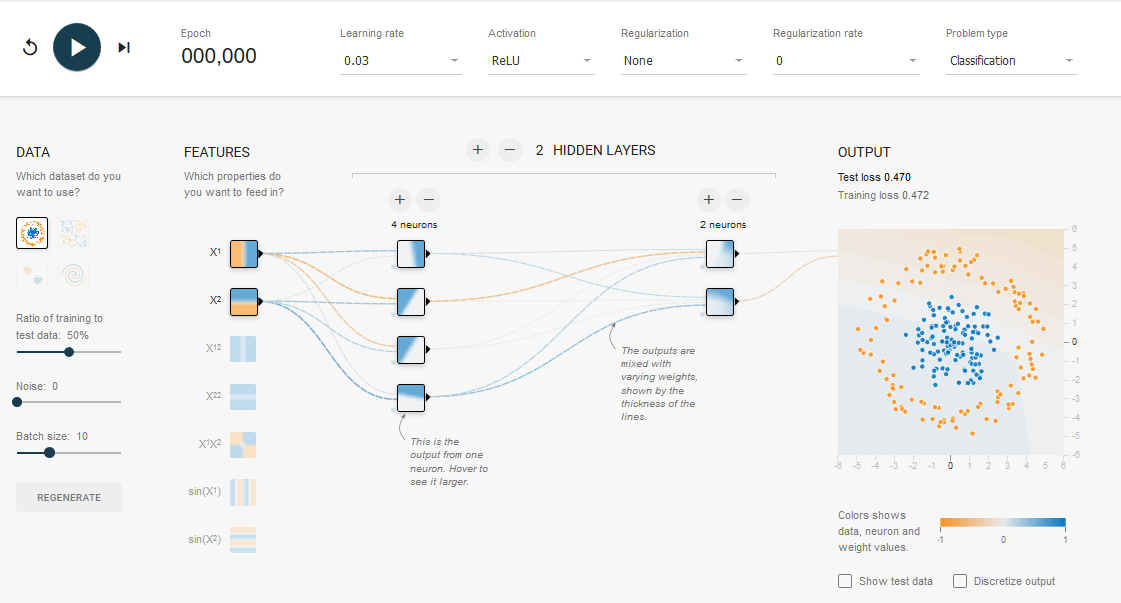
\includegraphics[scale=0.5]{../1ai_nn_start.png}
\end{figure}
\noindent
\noindent
\begin{figure}[H]
\centering
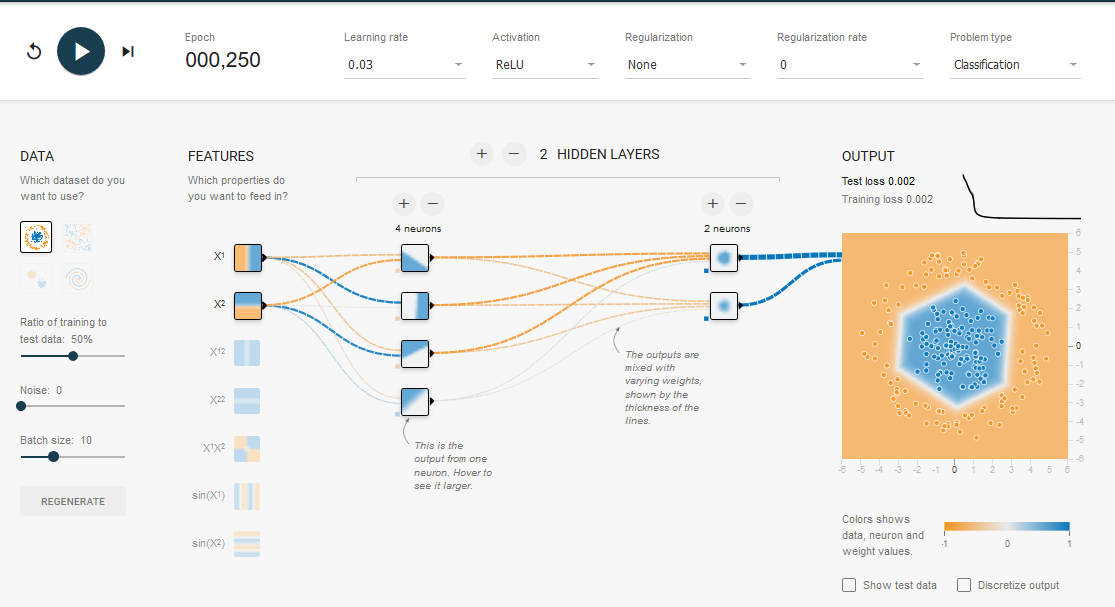
\includegraphics[scale=0.5]{../1ai_nn_end.png}
\end{figure}
\noindent
Since the weights for this model are initialized to be non-zero, the backpropagation algorithm is able to update the weights, along with the ReLU activation function being able to become nonzero from the weights. Thus, the model is able to converge to a solution with minimum trianing error.

\noindent
\begin{figure}[H]
\centering
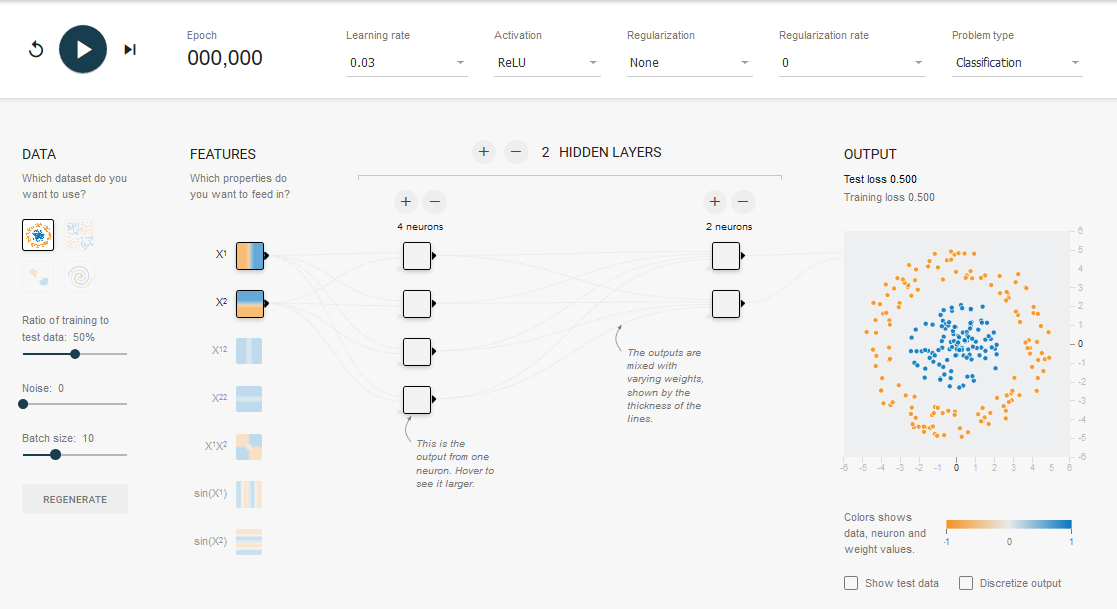
\includegraphics[scale=0.5]{../1aii_nn_start.png}
\end{figure}
\noindent
\noindent
\begin{figure}[H]
\centering
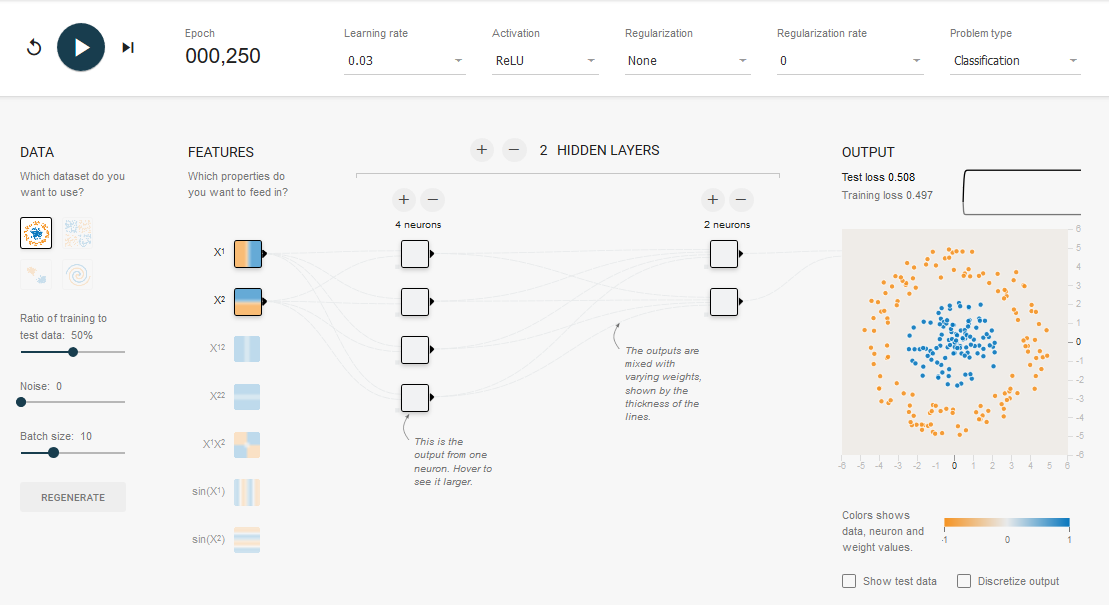
\includegraphics[scale=0.5]{../1aii_nn_end.png}
\end{figure}
\noindent
Since the weights for this model are initialized to be zero, the backpropagation algorithm is not able to update the weights from 0, along with the ReLU activation function always staying 0 from the weights which are all 0. Thus, the model is not able to converge to a solution with minimum trianing error.
}\end{solution}

\newpage
\problem[5] Backpropagation and Weight Initialization Part 2

\begin{solution}\normalfont{


\noindent
\begin{figure}[H]
\centering
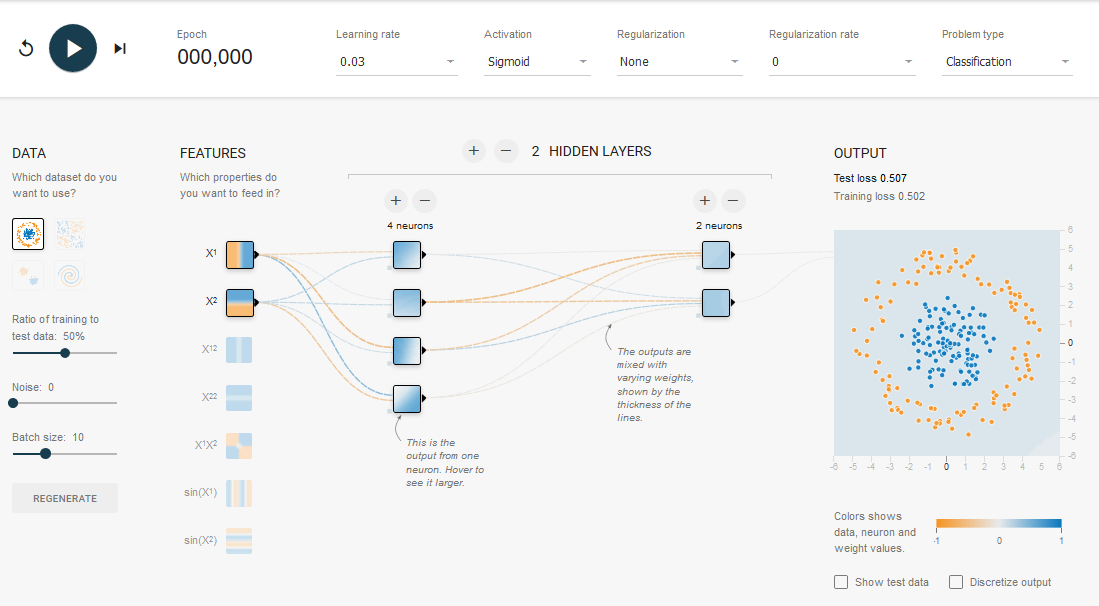
\includegraphics[scale=0.5]{../1bi_nn_start.png}
\end{figure}
\noindent
\noindent
\begin{figure}[H]
\centering
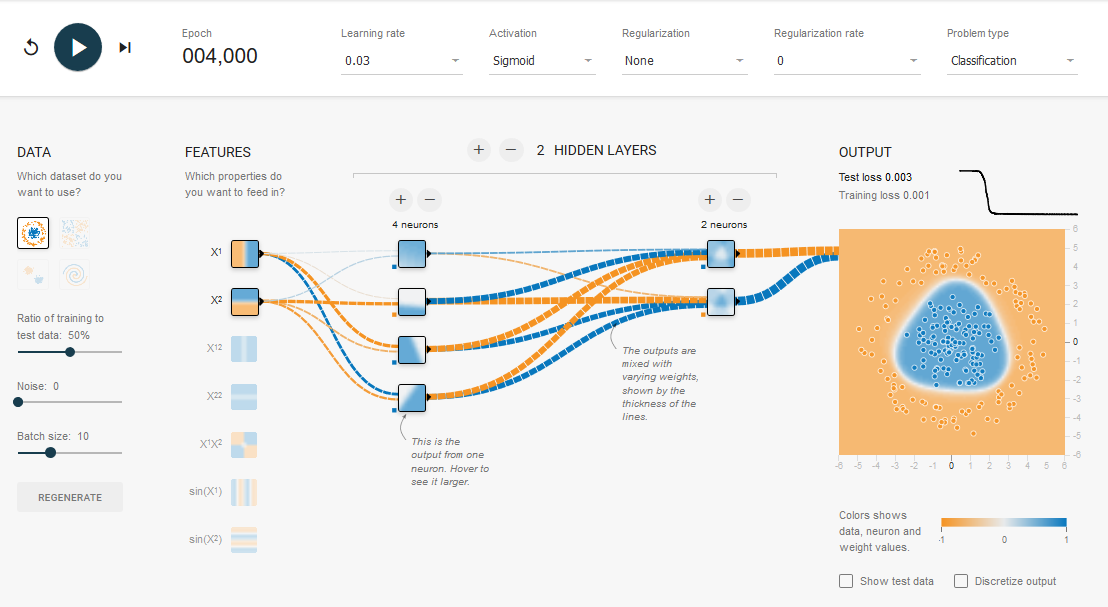
\includegraphics[scale=0.5]{../1bi_nn_end.png}
\end{figure}
\noindent
The neural network with nonzero-value initial weights learns the same as the corresponding neural network in Problem A, but this neural network learns at a much slower rate, since the sigmoid activation function $\sigma(x)$ approaches a derivative of 0 for large values of $x$.\\
\\
\noindent
\begin{figure}[H]
\centering
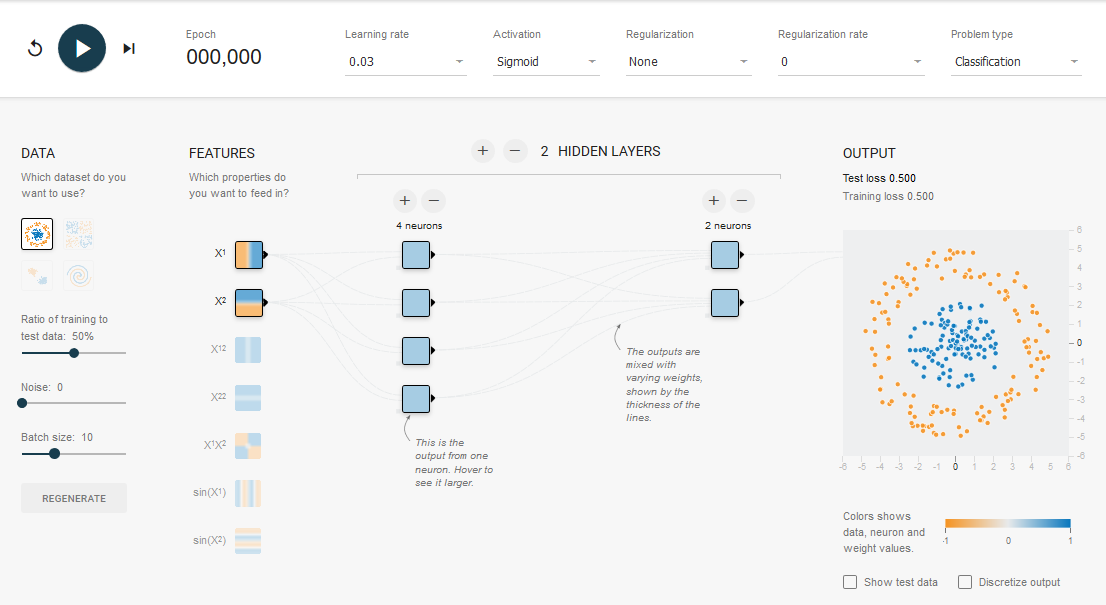
\includegraphics[scale=0.5]{../1bii_nn_start.png}
\end{figure}
\noindent
\noindent
\begin{figure}[H]
\centering
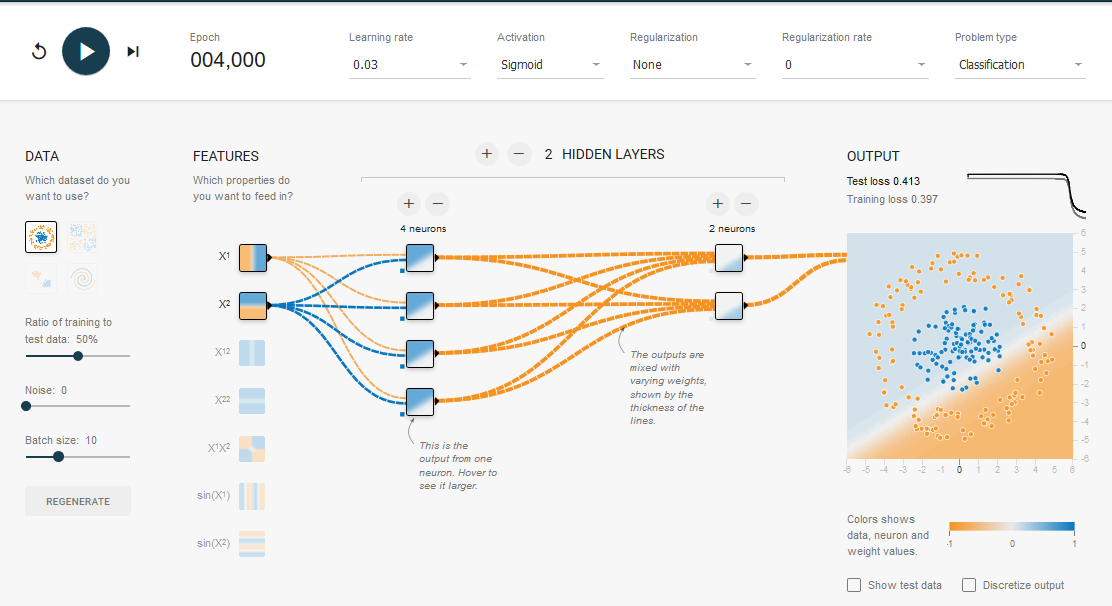
\includegraphics[scale=0.5]{../1bii_nn_end.png}
\end{figure}
\noindent
The neural network with zero-value initial weights learns a different model from that corresponding neural network in Problem A, as this model fits a line across the data, while the corresponding model does not fit any particular function to the data. This neural network learns at a slow rate, because even though the sigmoid function is nonzero at $x = 0$, the backpropagation algorithm updates weights close to 0 at a slow rate, along with the sigmoid function which converges slowly in general.
}\end{solution}


\newpage
\problem \textbf{[10 Points]}


\begin{solution}\normalfont{
If a fully-connected network with ReLU activations is trained using SGD looping through all the negative examples before any of the positive examples, then while the neural network is training on only negative examples first, the neural network will converge to fit only negative examples, which will cause some of the weights to become 0 and become impossible to update because ReLU activations cannot change zero-value weights. This makes the neural network unable to fit the positive examples next, because some of the weights of the neural network will be zero-value where they normally would not be to fit both the positive and negative examples (this is described by the dying ReLU problem).
}\end{solution}


\newpage
\problem[7] Approximating Functions Part 1

\begin{solution}\normalfont{
\noindent
\begin{figure}[H]
\centering
\includegraphics[scale=0.07]{../1d_nn.jpg}
\end{figure}
\noindent
The above neural network produces the OR function on two 0/1-valued inputs $x_1$ and $x_2$ using 0 hidden units, so this neural network uses the minimum number of hidden units to compute the OR function as described.
}\end{solution}

\newpage
\problem[8] Approximating Functions Part 2

\begin{solution}\normalfont{
\noindent
\begin{figure}[H]
\centering
\includegraphics[scale=0.07]{../1e_nn.jpg}
\end{figure}
\noindent
The above neural network produces the XOR function on two 0/1-valued inputs $x_1$ and $x_2$ using 2 hidden units. This neural network computes XOR by feeding the inputs and bias into the OR function (the top hidden unit), feeding the inputs and bias into the AND function (the bottom hidden unit), then subtracts the AND output from the OR output (this subtraction acts like applying NOT to the AND function output, so $(1,1)$ returns 0 from the neural network). For the $(0,0)$ input, the weights make AND function output -1, but the ReLU activation sets this value to 0. Since both hidden units are need for the calculation of XOR (one to compute OR and the other to compute AND), this neural network uses the minimum number of hidden units to compute the XOR function as described, so a network with fewer layers than 2 cannot compute XOR.
}\end{solution}
 

% problem 2
\newpage
\section{Depth vs Width on the MNIST Dataset  [25 Points]}

\problem \textbf{Installation} \textbf{[2 Points]}

\begin{solution}\normalfont{

Keras: 2.2.4

Tensorflow: protobuf-3.6.1 tensorflow-gpu-1.12.0

}\end{solution}

\newpage
\problem \textbf{The Data} \textbf{[1 Points]}

%\subproblem[1] The Data

\begin{solution}\normalfont{
The input data are images of handwitten numerical digits. The dimensions of the images are 28x28 pixels. High pixel values indicate where the digit is written in the image.
}\end{solution}

\newpage
%\subproblem[2]
\problem \textbf{One-Hot Encoding} \textbf{[2 Points]}
\begin{solution}\normalfont{
Shape of the training input: (60000, 784).
}\end{solution}

\newpage
\problem \textbf{Modeling Part 1} \textbf{[8 Points]}
\begin{solution}\normalfont{
(See 2_notebook for the model code.)\\
\\
Test accuracy: 0.9771.
}\end{solution}

\newpage
\problem \textbf{Modeling Part 2} \textbf{[6 Points]}

\begin{solution}\normalfont{
(See 2_notebook for the model code.)\\
\\
Test accuracy: 0.9801.
}\end{solution}

\newpage
\problem \textbf{Modeling Part 3} \textbf{[6 Points]}

\begin{solution}\normalfont{
(See 2_notebook for the model code.)\\
\\
Test accuracy: 0.9836.
}\end{solution}
 
 \newpage
 % problem 3
 \section{Convolutional Neural Networks  [40 Points]} 
 \problem Zero Padding \textbf{[5 Points]}

\begin{solution}\normalfont{
One advantage of zero-padding is that zero-padding can preserve the size of the input that the convolution operates on, which can make the convolution output easier to feed into another layer of the neural network (such as a dense layer of a neural network that works best with input sizes of powers of 2).\\
\\
One disadvantage of zero-padding is that zero-padding introduces noise into the convolution output, since the original data are augmented with the zero-padding to allow that convolution to preserve the size of the input with convolution.
}\end{solution}

\textbf{5 x 5 Convolutions}


\problem[2]

\begin{solution}\normalfont{
For each filter, there are $5 * 5 * 3$ parameters plus 1 bias term for a total of 76 parameters. Since there are 8 filters, there are $76 * 8 = 608$ parameters in total.
}\end{solution}

\problem[3] 

\begin{solution}\normalfont{
Since there is no zero-padding, the convolution runs on a tensor (the RGB image) the size of $28\times28\times3$, and since there are 8 filters, the shape of the output tensor is $28\times28\times8$.
}\end{solution}
 
\textbf{Max/Average Pooling}

\problem[3]

\begin{solution}\normalfont{
The average pooling matrices are as follows respectively to the original matrices:\\
$\begin{bmatrix}
    1 & 0.5 \\
    0.5 & 0.25 \\
\end{bmatrix}$,
$\begin{bmatrix}
    0.5 & 1 \\
    0.25 & 0.5 \\
\end{bmatrix}$,
$\begin{bmatrix}
    0.25 & 0.5 \\
    0.5 & 1 \\
\end{bmatrix}$, and
$\begin{bmatrix}
    0.5 & 0.25 \\
    1 & 0.5 \\
\end{bmatrix}$.
}\end{solution}

\problem[3]

\begin{solution}\normalfont{
The max pooling matrices are as follows respectively to the original matrices:\\
$\begin{bmatrix}
    1 & 1 \\
    1 & 1 \\
\end{bmatrix}$,
$\begin{bmatrix}
    1 & 1 \\
    1 & 1 \\
\end{bmatrix}$,
$\begin{bmatrix}
    1 & 1 \\
    1 & 1 \\
\end{bmatrix}$, and
$\begin{bmatrix}
    1 & 1 \\
    1 & 1 \\
\end{bmatrix}$.
}\end{solution}

\problem[4]

\begin{solution}\normalfont{
Pooling might be advantageous given these distortions in the dataset because pooling helps get rid of noise by smoothing the image slightly (in the case of average pooling), and by removing some pixels entirely (in the case of max pooling). Thus, pooling may help prevent a model from fitting to the noise of data, thus reducing overfitting for the model.
}\end{solution}

\problem[20] 

\subproblem[6, each 2]

\begin{solution}
%dropout layer immediately before final (output) layer in neural network

\end{solution}

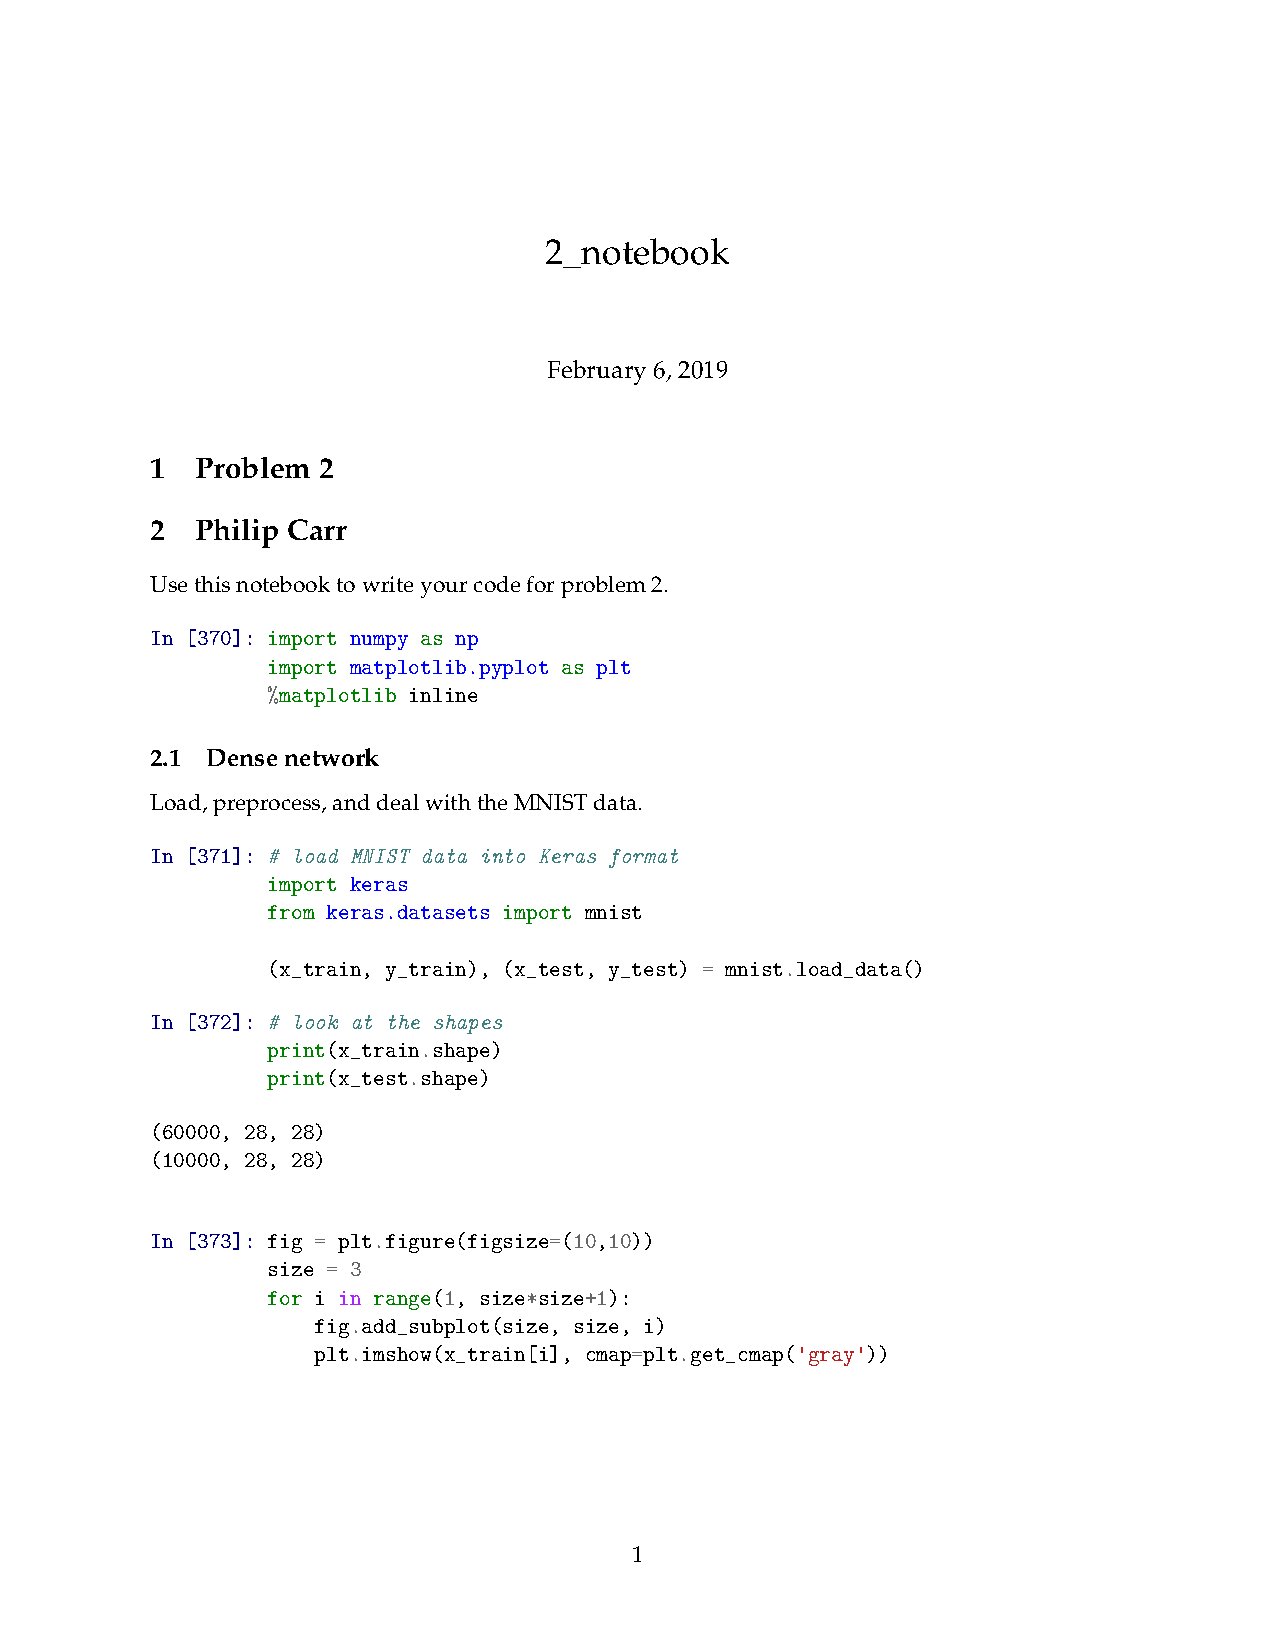
\includepdf[pages=-]{notebook2.pdf}

\end{document}
